%%%%%%%%%%%%%%%%%%%%%%%%%%%%%%%%%%%%%%%%%%%%%%%%%%%%%%%%%%%%%%%%%%%%%%%%%%%

\documentclass{standalone}

\usepackage{mathptmx}
\usepackage{tikz}
\usetikzlibrary{decorations.fractals}
\usetikzlibrary{external}
\tikzexternalize{koch-snowflake-1-area}

%% We default to Times.
\renewcommand{\rmdefault}{ptm}
\renewcommand{\ttdefault}{pcr}
%% Enable Times/Palatino main text font.
\normalfont\selectfont

%% The first iteration of the Koch snowflake.
\newcommand{\firstIteration}{%%
  %% Shade the known triangle.
  \draw[greyStyle] (origin) -- ++(\degree:\length) --
  ++(-\degree:\length) -- cycle;
  %% Draw the first iteration of the Koch snowflake.  Must be drawn last.
  \draw[lineStyle] decorate{%%
    (origin) -- ++(\degree:\length) -- ++(-\degree:\length) -- cycle%%
  }
  -- cycle;
}

%%%%%%%%%%%%%%%%%%%%%%%%%%%%%%%%%%%%%%%%%%%%%%%%%%%%%%%%%%%%%%%%%%%%%%%%%%%
%% The first iteration of the Koch snowflake.
%%%%%%%%%%%%%%%%%%%%%%%%%%%%%%%%%%%%%%%%%%%%%%%%%%%%%%%%%%%%%%%%%%%%%%%%%%%

\begin{document}

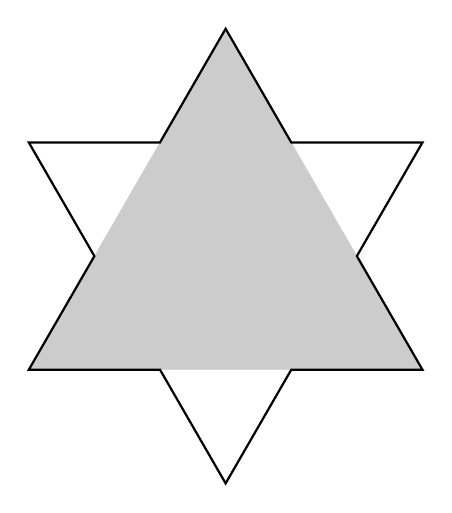
\begin{tikzpicture}[%%
  decoration=Koch snowflake,%%
  greyStyle/.style={-,ultra thin,fill=gray!40,gray!40},%%
  lineStyle/.style={-,thick}%%
]
%%
%%
\pgfmathsetmacro{\degree}{60}  %% Value of each internal angle.
\pgfmathsetmacro{\length}{5}   %% Length of each side of triangle.
\pgfmathsetmacro{\xlow}{0}
\pgfmathsetmacro{\ylow}{\xlow}
\coordinate (origin) at (\xlow,\ylow);
%%
%%
%% The first iteration of the Koch snowflake.
\firstIteration
\end{tikzpicture}

\end{document}
